
\documentclass[a4paper,11pt]{article}

\usepackage{amsmath,amssymb,amsfonts,amsthm}    % Typical maths resource packages
\usepackage{graphicx}                           % Packages to allow inclusion of graphics
\usepackage{hyperref}                           % For creating hyperlinks in cross references
\usepackage[authoryear]{natbib}                 % literature reference style
\usepackage[bf]{caption2}




% -------------------------------
% --- some layout definitions ---
% -------------------------------

% define topline
\usepackage[automark]{scrpage2}
\pagestyle{scrheadings}
\automark{section}
\clearscrheadings
\ohead{\headmark}

% define citation style
\bibliographystyle{ecta}

% define page size, margin size
\setlength{\headheight}{1.1\baselineskip}
\voffset=-2cm
\hoffset=-3cm
\textheight24cm
\textwidth15.5cm
\topmargin1cm
\oddsidemargin3cm
\evensidemargin3cm

% define line line spacing = 1.5
\renewcommand{\baselinestretch}{1.5}

% define second level for `itemizing'
\renewcommand{\labelitemii}{-}



\begin{document}

% -------------------------------
% --- frontmatter: Title page ---
% -------------------------------

\thispagestyle{empty}
\begin{center}

    {\Large{\bf Random Number Generation}} \vspace{0.5cm}



    \bigskip
    \bigskip

    {\normalsize by \\\vspace{0.5cm}
    {\bf Yinan Wu} \\
    (519164)} \vspace{1cm}


    {\normalsize for the Numerical Introductory Course (WS 15/16)\\
    {\bf Master of Science} \\
    Berlin, Feb 27, 2016}

\end{center}





% -----------------------------
% --- frontmatter: Abstract ---
% -----------------------------
\newpage
\section*{Abstract}

This report is about the basic principles and methods for the random number generators used in simulation. The emphasis is on the methods of uniform random generators, which can be later transformed to other sequence of numbers following different distribution. we consider the linear recurrence as a easy mathematical structure for building a uniform random number sequence. This methodology is convenient to be understood and applied, and this is also one of the most common generators used in simulation. Secondly, we will discuss 
the non-uniform random generators. The algorithms include the inverse method, Box-Muller Method. Finally, we will discuss the statistical testing to verify whether our generator is appropriate or not.\\

Keywords: random number generator, linear congruential generator, uniform random generator, the inverse method, box-muller method, statistical test. \\



% -----------------------------
% --- frontmatter: Contents ---
% -----------------------------
\newpage
\tableofcontents
\clearpage



% -------------------------------
% --- main body of the thesis ---
% -------------------------------
\newpage
\pagestyle{plain}
\setcounter{page}{1}    % start page numbering anew
\pagenumbering{arabic}  % page numbers in arabic style


\section{Introduction}

Random numbers refers to "a sequence of independent numbers with a specified distribution and a specified probability of falling in any given range of values" (The Art of Computer Programming, Volume 2, Donald E. Knuth). A pseudo random number generator (RNG) is a basic and important component for a stochastic simulation. The mathematical theoretical background is built over the concepts of probability and random variable. However, since the exact implementation of those concepts on conventional computers are impossible, random variables and other random objects are in fact simulated by deterministic algorithms. Non-uniform random variate generation is concerned with certain distributions. Such random variables can be discrete or continuous, and it is described by density function. Random variate generation for simulation can be decomposed in two steps: generating restrictions of independent and identically distributed (i.i.d) random variables having the uniform distribution over the interval (0,1), then applying transformations to those i.i.d  $U$ random variates to generate random variates and random vectors from arbitrary distributions, such like Gaussian distribution. The generation of Gaussian random number is the essential simulation of many financial problems. we will discuss later methods for getting Gaussian random numbers, one of which works by transforming uniformly distributed numbers using Box-Muller method.\\

In fact, we have found out that random numbers have several applications. 
\begin{itemize}
\item{Music and Graphics Composition: By interweaving content with random bits, the result can be used in image processing and reconstruction, electronic music composition, and 3-D texturing techniques for computer graphics.}
\item{Equation-Solving: Mathematicians use random numbers to help them solve complex equations.}
\item{Entertainment: Modern lotteries and gambling machines are all based on the use of random numbers. Video games use random numbers to influence intelligence heuristics or to vary game play. }
\item{Cryptography, Digital Signatures, Protected Communication Protocols: Because of computer security, there is a growing interest in random number generation due to their value in key generation for cryptography, digital signatures, and protected communication protocols. At the base of these techniques used to secure data and data transmissions lies key generation, which requires the production of secret, unguessable keys. Hence, key generation depends on an RNG to provide the required entropy to make the key indeterminable. Increased computer security enables businesses to take advantage of enhanced network services such as remote access and e-Business. With  enhanced computer security, consumers obtain better and more convenient access to electronically available products and services such as shopping on-line, banking at-home, and downloading protected content. }
\end{itemize}
One of the other applications for RNG is option pricing. The most common model for stocks follows geometric Brownian motion, which assumes that the percentage changes in a stock's price follows the Gaussian distribution, where the final price of the stock at time $t$ is defined as $S_t = S_0e^{(u+sN)}$. There are two characteristics of stock price, prices are never negative, and the magnitude of stock price fluctuations is proportional to the magnitude of the stock price. The simple option price and be determined in some ways: Black-Scholes pricing formula, finite-difference methods, binomial trees, or Monte Carlo simulation. Additionally, random number generation has also other applications.  \\ 

At the end, due to the mathematical evaluation of randomness is difficult, we can use statistical analyses on the generated sequences to detect the characteristics of randomness,
which is in the last chapter. 
\\

\section{Uniform Random Number Generators}
{RNGs used for simulation are almost always based on some deterministic algorithms that, 

\subsection{Linear Congruential Generator}
{The classic generator is the linear congruential generator (LCG) (Knuth 1969). This is also the oldest in common use, which uses a transition function of the form
\begin{center} $X_{n+1}=aX{n}+c$ mod $m$, $n>0$. 
\end{center}
The maximum period of the generator is $m$, but the longest period can be at most $2^{32}$. The linear congruential generator also have statistical 
drawbacks, which make themselves unsuitable for simulations. There are three particular problem with LCG. One serious flaw is that plotting. It display an obvious lattice 
structure. Another problem is that the periods of LCG generators are often too short. The period of LCG depends on the $m$, The The maximum period of the generator 
is $m$ for the first class; $2^{N-2}$ for second class; $m-1$ for third class (Anderson, 1990). The LCG generators are not the best random number generators. 
They are still very good. Knuth considers it the nicest and simplest random number generator for the machine language of most computers.
}
\subsection{Combined Linear Congruential Generator}
{A derivate of the LCG is the multiple recursive generator (MRG), which combines two or more generators. These generators provide both good statistical quality and long periods.\\
Here is a example:\\
Set
$X_{1,0},X_{1,1},X_{1,2},X_{2,0},X_{2,1},X_{2,2}$,For $i\geqslant 3$,set\\
$X_{1,i}$=(1,403,580 $X_{1,i-2}$-810,728 $X_{1,i-3}$) mod(2^{32}-209)\\
$X_{2,i}$=(527,612 $X_{2,i-1}$-1,370,589 $X_{2,i-3}$) mod(2^{32}-22,853)\\
$Y_i$=$(X_{1,i}-X_{2,i})$ mod(2^{32}-209)\\
$U_i$=$Y_i$/(2^{32}-209)\\
 
 A particularly well-known combination generator is Numerical Recipes? RAN2 [Presset al., 1992]. This is their 1,000.00 generator, for which they will give 1,000.00 to the first reader who finds a statistical test that RAN2 fails in a non-trivial way, excluding the ordinary limitations of a machine floating point representation. This generator combines two linear congruential generators and further randomizes by shuffing.
}



\subsection{Lagged Fibonacci Generator}
A Lagged Fibonacci Generator is an example of a pseudo random number generator. This class of generator aims to be an improvement on the the stand LCG. 
{\begin{center}
$X_i=(X_{i-r}opX_{i-s})$ mod $m$,\\the possible operations can be addition and multiplication \\
\end{center}
where $U_i=X_i/m$ $m$ is the modulus,$X_0,X_1$ are seeds.\\

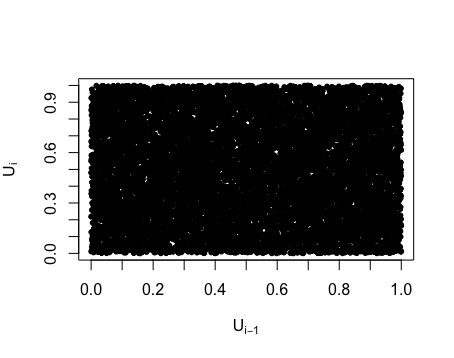
\includegraphics[scale=0.8]{fb}\\

 LFG (Knuth 1969) is used commonly in distributed Monto Carlo simulations. This generator is similar to an LCG but introduces a delayed feedback. However, to achieve good quality, the constant $k$ must be large. Consequentially $k$ words of memory must be used to hold the state. Typically
$k$ must be greater than 1000, and each thread will require its own state, so this must be stored in global memory. We thus reject the lagged Fibonacci method but note that it
may be useful, because of the simplicity and small number of registers required.  The multiplication generator has been shown to have very good properties. It was the only 
generator besides some combination generators to pass all Diehard test. 

}

\subsection{Tausworthe Generator}
{Tausworthe (1965) introduced a generator based on a sequence of 0 and 1 generated by a recurrence of the form\\
Define a sequence of binary digits $B_1,B_2,...$by\\
\begin{center}
$B_i=(\sum_{j=1}^qc_jB_{i-j})$mod 2,\\
\end{center}
where $c_i$=0 or 1\\
Usually \\
\begin{center}
$B_i=(B_{i-r}+B_{i-q})$mod 2,($0\<r\<q$)\\
\end{center}
}



}
 
\section{Non-uniform Random Number Generators}
{Like for the uniform case, non-uniform variate generation often involves approximations and compromise. The does not mean that the generated random variate $X$ must
always have exactly the required distribution, because this would sometimes be much too costly or even impossible. But we must have a good approximation. 
\subsection{The Inverse Method}
{The inversion can be a good choice for obtaining non-uniform random variates in a majority of situations. The fact that $X=F^{-1}(U)$ is a monotone function of $U$ makes the method
compatible with important variance reduction techniques. For some distributions, an analytic expression can be obtained for the inverse distribution function $F^{-1}$ and inversion 
can be easily implemented. For example, consider the Exponential distribution function with parameter $\lamda > 0$, $x=F^{-1}(y)=-\frac{ln(1-y)}{\lambda}$, $y\in[0,1)$. \\
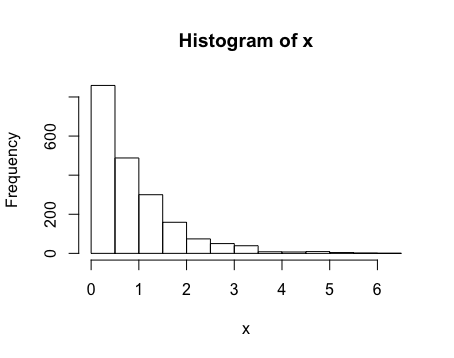
\includegraphics[scale=0.8]{in}\\
However, there are other distributions (e.g., the normal, Student, chi-square), which do not have closed-form expression for $F^{-1}$.  When the distribution has only scale and location parameters, we need to approximate $F^{-1}$ only for a standardized version of the distribution, such as normal distribution. When shape parameters are involved (e.g., the gamma and beta distributions), things are more complicated because  $F^{-1}$ depends on the parameters in a more fundamental manner.\\
}
\subsection{Types of Gaussian Transforms}
{
\subsubsection{The Ziggurat Method}
{The fast method in software is the Ziggurat method (Marsaglia 2000). This procedure uses a complicated method to split the Gaussian probability density function into rectangles, 
and it is designed to minimize the average cost of generating a sample. However, this means that for 2 percentage of generated numbers, a more complicated route using further 
uniform samples and function calls must be made. In software this is acceptable, but in fact the performance of the slow route will apply to all threads in a warp.

}
\subsubsection{Box-Muller Method}
{The Box-Muller Transform, by George Edward Pelham Box and Mervin Edgar Muller 1958, is a pseudo-random number sampling method for generating pairs of independent, standard
normally, distributed random numbers, given a source of uniformly distributed random numbers. It turns out that one of the best choice for the Gaussian transform is actually the 
venerable Box-Muller transform. The form
Suppose $U_1$ and $U_2$ are independent random variables that are uniformly distributed in the interval (0,1). Let\\
\begin{center}
$y_1=\sqrt{-2logx_1}cos2\pi x_2=h_1(x_1,x_2)$\\
$y_2=\sqrt{-2logx_1}sin2\pi x_2=h_2(x_1,x_2)$\\}
\end{center}
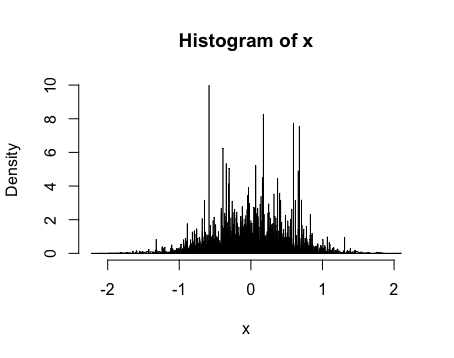
\includegraphics[scale=0.8]{bm}\\
The Box-Muller method is not widely used in software, because it involves sine and cosine for producing the sample. 
}

}
}
\section{Statistic Testing} 
{Before computers, scientists typically rolled dice, tossed coins, or drew cards to provide random numbers. The first tests for random numbers were published by M.G. Kendall and Bernard Babington Smith in the Journal of the Royal Statistical Society in 1938. They were built on statistical tools such as Pearson's chi-squared test that were developed to distinguish whether experimental phenomena matched their theoretical probabilities. Pearson developed his test originally by showing that a number of dice experiments by W.F.R. Weldon did not display "random" behavior. With the introduction of computers, the scientific community pushed the development of mathematical algorithms for random number generation to be used in scientific simulation, software testing, and mathematical modeling. As these algorithms were developed, problems arose from using algorithms that produced sequences containing patterns or that generated certain numbers more than others. To test the strength of various algorithms, Dr. George Marsaglia of Florida State University invented the Diehard test suite which contains a battery of statistical tests focused on weeding out PRNGs that have a short period, patterns within the bits, and non-uniform distribution of numbers. \\

\subsection{The $\chi^2$ Goodness-of-Fit Test}
{
The chi-square test is listed by Knuth (1981) as a good statistical test of a random number generator. The basic idea behind the test is as follows.\\
Divide the unit interval into $k$ cells, like $[0,\frac{1}{k}),[\frac{1}{k},\frac{2}{k})...[\frac{k-1}{k},1]$. For a uniform distribution, then a particular observation 
$R_j$ will fall into a cell with probability $ \frac{1}{k}$.\\
$O_i$ counts $R_j$ felled into cell $i$, $O_i$ \sim Bin(n,\frac{1}{k}), \\
\smallskip
\textbf{The $\chi^2$ goodness-of-fit statistic is},\\
\begin{center}
$\chi_0^2$=$\sum_{i=1}^k \frac{(O_i-E_i)^2}{E_i}$\\
\end{center}
where $E_i=\mathbb{E}[O_i]=n/k$\\
\smallskip
if $\chi_0^2<\chi_{\alpha,k-1}^2$, we fail to reject $H_0$.\\}
\subsection{The Kolmogorov-Smirnov Test}
{This test is designed to test quantities that fall into a finite number of categories.Random numbers are expected to have continuous distributions. A good test for continuous distributions is the Kolmogorov-Smirnov (K-S) test (Knuth, 1981). For a distribution that has a cumulative distribution function, F, with no jumps (i.e. the distribution is continuous), the values $K^+_n$ and $K^-_n$ are de?ned as:
\begin{center}
$K^+_n= \sqrt(n) max(F_n(x)-F(x))$\\
$K^-_n=  \sqrt(n) max(F(x)-F_n(x))$\\
\end{center}
where n is the number of values being tested, Fn is the cumulative distribution function calculated from these values and F is the theoretical value of this cumulative distribution function. For a uniform distribution, F(x) = x.
}
\subsection{Runs Test for Independence}
{The runs test (also called Wald-Wolfowitz test after Abraham Wald and Jacob Wolfowitz) is a non-parametric statistical test that checks a randomness hypothesis for a two-valued data sequence. More precisely, it can be used to test the hypothesis that the elements of the sequence are mutually independent.\\

A "run" of a sequence is a maximal non-empty segment of the sequence consisting of adjacent equal elements. For example, the 22-element-long sequence "++++---+++--++++++----" consists of 6 runs, 3 of which consist of "+" and the others of "-". The run test is based on the null hypothesis that each element in the sequence is independently drawn from the same distribution.\\
Runs test can be used to test: randomness of a distribution, by taking the data in the given order and marking with + the data greater than the median, and with - the data less than the
median; (Numbers equalling the median are omitted.). The hypothesis of statistical independence of the elements may be rejected, if the number of runs is significantly higher or lower than expected. \\
If $n$ is large(at least 20) and the $R_i$ are actually independent, $L$ is the number of runs, then\\
\begin{center}
$L$ \sim N(\frac{2n-1}{3},\frac{16n-29}{90})\\
\end{center}
Example:\\
 if $n$=60, we could expect there are around 40 runs,variance is 10.3. \\
If $\alpha=0.05$, $z_0$=1.96, So we expect to see, \\ Confidence interval: 40$\pm$1.96\sqrt{10.3}\sim [33,71,46.29]\\
}
}

\section{Conclusion}
{
The ultimate goal of RNG structure is to obtain a fast algorithm, whose output cannot 
be distinguished in any way from a realization of an infinite sequence of 
i.i.d uniform variables. This requirement is that, the generated sequence of numbers need to be statistical significant, which 
in general means uniformity and independence. It seems that this can come out through a physical device 
based on quantum physics. There may exist some problems, one of them being that the sequence 
cannot be reproduced without storing.\\
 

RNGs based on linear recurrences and output transformations, 
are known to fail statistical tests of linear 
complexity, even when their period length is 
huge. This seems to have no impact for the great majority of 
relevant discrete-event simulation applications, but it would nevertheless 
be good to have efficient alternative non-linear RNGs that also
pass these linear complexity test. \\

For the development of huge period lengths (e.g., near $2^{20000}$ or even more) with huge \
period lengths as well as faster generators based.\\

Poor (or plain bad) generators can still be found in popular commercial  
statistical and simulation software, spreadsheets, etc. For example the the famous 
Randu Random generator. We are also not satisfied with those numbers that are in software package. An important task
of RNG experts is to study these proposals carefully to shed light on their potential weakness.\\
}


% literature
\newpage
\addcontentsline{toc}{section}{References}

\begin{thebibliography}
 Eichenauer-Herrmann, J. (1995). Pseudo random number generation by non-linear methods. International Statistical Reviews.\\
 Gentle, J. E.(2003). Random Number Generation and Monte Carlo Methods. Springer, NewYork, second edition.\\
 L Ecuyer, P.(1990). Random numbers for simulation. Communications of the ACM, 33(10).\\
 L Ecuyer, P.(1998). Random number generation. In Banks,J., editor, Hand-book of Simulation, Wiley. chapter4.\\
 Marsaglia, G. and Zaman, A.(1991).A new class of random number generators. The Annals of Applied Probability.\\
 L Ecuyer, P., Hellekalek, P., 1998. Random number generators: Selection criteria and testing. In: Hellekalek, P., Larcher, G. (Eds.), Random and Quasi-Random PointSets. Vol.138 of Lecture Notes in Statistics. Springer, NewYork.\\
 Leeb,H.,1995. Random numbers for computer simulation. Master thesis, University of Salzburg.\\
 Tausworthe, R. C., 1965. Random numbers generated by linear recurrence modulo two. Mathematics of Computation 19.\\
 L. Devroye, Random variate generation for unimodal and monotone densities, Computing,vol.32, 1984b.\\
Marsaglia, G., 1996. The Marsaglia random number CDROM including the DIEHARD battery of tests of randomness, see http://stat.fsu.edu/pub/diehard.\\
 
 
 
 
\end{thebibliography}


\end{document}
